\documentclass[aspectratio=1610,11pt]{beamer}
\definecolor{spoiler}{gray}{0.6}

\usepackage[utf8x]{inputenc}
\usepackage[T2A]{fontenc}
\usepackage[russian]{babel}
\usepackage{xcolor}
\usepackage{MnSymbol}
\usepackage{mathrsfs}
\usepackage{listings}
\usepackage{mathtools}
\usepackage{amssymb,amsmath, dsfont, amsthm}
\usepackage{hyperref}
\hypersetup{unicode=true}
\usepackage{comment}
\usepackage{graphicx}
\usepackage{tikz,makecell}
\usepackage{wrapfig}
\usepackage{xfrac}
\usepackage{qrcode}

\usetheme{Berlin}

\usecolortheme{dolphin}
\title[Разделяй и\ldots достаточно]
	{\bfseries Разделяй и\ldots\ достаточно}
\author[Тодоров Е.И.]{Тодоров Е.И.}
\institute[Санкт-Петербургский Турнир юных математиков, Фонд <<Время науки>>]{\large Санкт-Петербургский Турнир юных математиков, Фонд <<Время науки>>}
\date{\today}

\newtheorem{Th}{Теорема}
\newtheorem{Le}{Лемма}
\newtheorem{Def}{Определение}
\newtheorem{Ex}{Пример}
\newtheorem{Proposition}{Предложения}
\newtheorem{Property}{Свойство}
\newtheorem{Prof}{Доказательство}
\newtheorem{Profcont}{Доказательство (продолжение)}
\newtheorem{Exer}{Упражнение}

\newcommand\fram[2]{\begin{frame}{\bf #1} #2 \end{frame}}
\newcommand\framm[1]{\begin{frame} #1 \end{frame}}
\newcommand{\comm}[1]{$\backslash$\texttt{#1}}
\def\scolon{\rlap{,}\raisebox{0.8ex}{,} }
\def\mitem{\medskip\item}
\newcommand{\myref}[2]{\href{#1}{\texttt{\underline{#2}}}}
\newcommand{\set}[1]{\left\{ #1 \right\}}

\def\divsby{\mathop{\rlap{.}\rlap{\raisebox{0.55ex}{.}}\raisebox{1.1ex}{.}}}
\def\usl#1#2{\begin{block}{#1} #2 \end{block} \medskip\pause}
\def\uslnp#1#2{\begin{block}{#1} #2 \end{block} \medskip}

\newcommand{\hackcenter}[1]{
 \xy (0,0)*{#1}; \endxy}
\newcommand{\scs}{\scriptstyle}
\newcommand{\xsum}[2]{
 \xy
 (0,.4)*{\sum};
 (0,3.7)*{\scs #2};
 (0,-2.9)*{\scs #1};
 \endxy
}
\newcommand{\refequal}[1]{\xy {\ar@{=}^{#1}
(-1,0)*{};(1,0)*{}};
\endxy}

\usepackage[linguistics]{forest}

\newcommand{\fstfor}[5]{
	\begin{figure}[h] \centering
	\begin{forest} for tree={circle, draw, minimum size=1.7ex, inner sep=0.45pt,% 
	   l=#2cm, s sep=#3mm}
		#1
	\end{forest}
		\caption{#4} \label{#5}
	\end{figure}}


\begin{document}
\section{ }
\begin{frame}\titlepage\end{frame}

\fram{Эта презентация онлайн}{
\Large
\begin{center}
Зачем фотографировать презентацию, \\
		когда её можно скачать? \\[0.3cm]
		\qrcode[height=4cm]{http://bit.ly/about_division} \\[0.3cm]
		\url{http://bit.ly/about_division}
\end{center}
}

\section{Делимость}
\fram{Определение деления}{
\large
\begin{Def}
Для целых чисел $a$ и $b$ будем говорить, что $a$ делится на $b$, если существует такое целое число $n$, что $a = nb$. Будем писать $a \divsby b$.\\
Число $b$ в этом случае называется делителем $a$.
\end{Def}
Свойства делимости:
\begin{itemize}
\item для любого целого $a$ выполнено $0 \divsby a$;
\item если $a \divsby b$ и $b \divsby c$, то $a \divsby c$;
\item если $ac \divsby bc$ и $c \ne 0$, то $a \divsby b$;
\item если $(a+b) \divsby c$ и $a \divsby c$, то $b \divsby c$.
\end{itemize}
}

\fram{Определение деления с остатком}{
\large
\begin{Def}
Для целых чисел $a$, $b$ и $r$ ($0<r<b-1$) будем говорить, что $a$ делится на $b$ с остатком $r$, если существует такое целое число $n$, что $a = nb+r$ и $r$ --- наименьшее из таких чисел.
\end{Def}

\begin{Property}
Разность $(a-b)$ делится на $c$ тогда и только тогда, когда остатки от деления $a$ и $b$ на $c$ одинаковые.
\end{Property}
}

\fram{Упражнения}{
\large
\begin{Exer}
Найдите наибольшее четырёхзначное число, которое делится на 31.
\end{Exer}

\begin{Exer}
Число $100$ разделили на некоторое число $n < 50$ и получили остаток 6. Найдите $n$.
\end{Exer}

\begin{Exer}
Может ли некоторое число делиться на $8$, а при делении на $12$ давать остаток $10$?
\end{Exer}
}

\section{НОД}
\fram{Определение НОД}{
\large
\begin{Def}
Целое число $D$ называется наибольшим общим делителем чисел $a$ и $b$, если выполнены свойства:
\begin{enumerate}
\item $D$ является делителем $a$ и $b$: $a \divsby D$ и $b \divsby D$;
\item $D$ делится на любой другой делитель $a$ и $b$: для любого $d$ если $a \divsby d$ и $b \divsby d$, то $D \divsby d$.
\end{enumerate}
В этом случае пишут $D= \NOD(a, b)$.
\end{Def}
\begin{Property}
Для любого целого $a$ выполнено $\NOD(a, 0) = a$.
\end{Property}
}


\fram{Наивные методы поиска НОД}{
\large
\begin{enumerate}
\item Перебрать все числа до $\min(a, b)$.
\begin{Exer}
Найдите $\NOD (12, 16)$ и $\NOD (15, 21)$.
\end{Exer} \pause
\item Выписать все простые делители $a$ и $b$, а затем найти общие и перемножить их.
\begin{Exer}
Найдите $\NOD (12, 16)$, $\NOD (15, 87)$ и $\NOD (60, 210)$.
\end{Exer}
\end{enumerate}
}

\fram{Лемма об общем НОД}{
\large
\begin{Le}
Для целых чисел $b$, $n$ и $r$ имеет место равенство $\NOD(b,r) = \NOD(bn+r, b)$.
\end{Le}

\begin{Prof}
Нетрудно видеть, что \[ \NOD(b,r) \divsby \NOD(bn+r, b)\] \pause и, наоборот, \[\NOD(bn+r, b) \divsby \NOD(b,r).\] \pause А значит, $\NOD(b,r) = \NOD(bn+r, b)$
\end{Prof}
}

\fram{Об остатках и разности}{
\large
\begin{Property}
Найти остаток $r$ от деления числа $a$ на число $b$ можно, вычитая $b$ из $a$, \linebreak пока это возможно.
\end{Property}

\begin{Ex}
Найдём остаток от деления числа $85$ на $16$:
\begin{enumerate}
\item $85 -16 = 69$;
\item $69 -16 = 53$;
\item $53 -16 = 37$;
\item $37 -16 = 21$;
\item $21 -16 = 5$.
\end{enumerate}
\end{Ex}
}

\section{Алгоритм Евклида}
\fram{Алгоритм Евклида}{
$\NOD(a, b)$ для $a>b$ может быть найден благодаря следующему алгоритму, в котором последовательно находятся числа $q$ и $r$:
\begin{align*}
a = bq_1+r_2, && 0 < r_2 < b \\
b = r_2q_2+r_3, && 0 < r_3 < r_2 \\
r_2 = r_3q_3+r_4, && 0 < r_4 < r_3 \\
\vdots && \vdots \\
r_{n-3} = r_{n-2}q_{n-2}+r_{n-1}, && 0 < r_{n-1} < r_{n-2} \\
r_{n-2} = r_{n-1}q_{n-1}+r_n, && 0 < r_n < r_{n-1} \\
r_{n-1} = r_{r_n}q_n. && \\
\end{align*}
Этот алгоритм продолжается до тех пор, пока на некотором шаге число $r_{n+1}$ не станет равно 0.
}

\fram{Пример и упражнения}{
\large
\begin{Ex}
Найдём $\NOD(100, 44)$:\pause
\begin{enumerate}
\item $100 = 44\cdot2 + 12$ ($q_1= 2$, $r_2= 12$);\pause
\item $44= 12\cdot3+8$ ($q_2= 3$, $r_3= 8$);\pause
\item $12 = 8\cdot1+4$ ($q_3= 1$, $r_4= 4$);\pause
\item $8 = 4\cdot2$ ($q_4= 2$, $r_5= 0$).
\end{enumerate}
То есть $\NOD(100, 44) = 4$.
\end{Ex}

\begin{Exer}
Найдите $\NOD(108, 48)$, $\NOD(72, 42)$ и $\NOD(34, 21)$.
\end{Exer}
}

\fram{О конечности алгоритма Евклида}{
\Large
Заметим, что на кажом шаге мы работаем с числами, становящимися всё меньше и меньше: $$b >r_2>r_3>r_4>\ldots$$
Поскольку мы работаем с натуральными числами, этот процесс обязательно когда-то закончится.
}

\fram{О линейном выражении НОД}{
\large
С помощью алгоритма Евклида мы можем линейно выразить $\NOD(a,b)$ через числа $a$ и $b$, то есть подобрать такие целые числа $m$ и $n$, что $\NOD(a,b) = ma+nb$.
\begin{Ex}
Найдём $\NOD(98, 21)$:
\begin{enumerate}
\item $98 = 21\cdot4 + 14$ ($q_1= 4$, $r_2= 14$);
\item $21= 14\cdot1+7$ ($q_2= 1$, $r_3= 7$);
\item $14 = 7\cdot2$ ($q_3= 2$, $r_4= 0$).
\end{enumerate}
То есть $\NOD(98, 21) = 7$.\\
$\NOD(98, 21) = 7 = 21-14 = 21-(98-21\cdot4) = (-1)\cdot98+5\cdot21$.
\end{Ex}
}

\fram{Упражнения}{
\Large
\begin{Exer}
\begin{enumerate}
\item Выразите $\NOD(20, 12)$ через $20$ и $12$;
\item Выразите $\NOD(72, 32)$ через $72$ и $32$;
\item Выразите $\NOD(153, 54)$ через $153$ и $54$.
\end{enumerate}
\end{Exer}
}

\fram{Диофантовы уравнения}{
\Large
\begin{Th}
Для целых $a$, $b$ и $c$ линейное уравнение $ax+by = c$ имеет решение в целых тогда и только тогда, когда $c \divsby \NOD(a, b)$, то есть если существует такое целое $t$, что $c = t\cdot\NOD(a,b)$.
\end{Th}
\begin{Prof}
Поскольку $\NOD(a,b)$ линейно выражается через $a$ и $b$: $ma+nb=\NOD(a,b)$ --- имеет место равенство $t\cdot ma+t\cdot nb=t\cdot\NOD(a,b)$ или $tm\cdot a + tn\cdot b = c$. Значит, достаточно просто взять $x = tm$ и $y = tn$.
\end{Prof}
}

%\section{Цепные дроби}
%\fram{Определение цепной дроби}{
%ыть
%}

%\fram{Примеры цепных дробей}{
%ыть
%}

%\fram{Связь цепных дробей и алгоритма Евклида}{
%ыть
%}

%\fram{Упражнения}{
%ыть
%}

\section{Летний ТЮМ}
\fram{Летний Турнир для 5--7 классов}{
\Large
\begin{itemize}
	\item пройдёт очно со 2 по 8 августа;
	\item участие и проживание бесплатно для участников;
	\item новый формат, сочетающий особенности Турнира и Регаты;
	\item 3 серии нестандартных задач;
	\item по 1.5 дня на решение;
	\item устный доклад в формате мат.боя на 2 команды.
\end{itemize}
}

\fram{Регистрация на Летний Турнир}{
\Large
\begin{center}
	Зарегистрировать команду на\\ Летний Турнир юных математиков:\vspace{0.2cm}
	
	\qrcode[height=4cm]{https://forms.gle/5fAsDNECis7aFZKT8}\vspace{3mm}
		
	\url{spbtym.ru} $\rightarrow$ Зарегистрироваться
\end{center}
}


\framm{
\begin{center}
\begin{tabular}{lcr}
\makecell[c]{
\includegraphics[width=0.3\textwidth]{pgrants_logo.png}} &
\makecell[c]{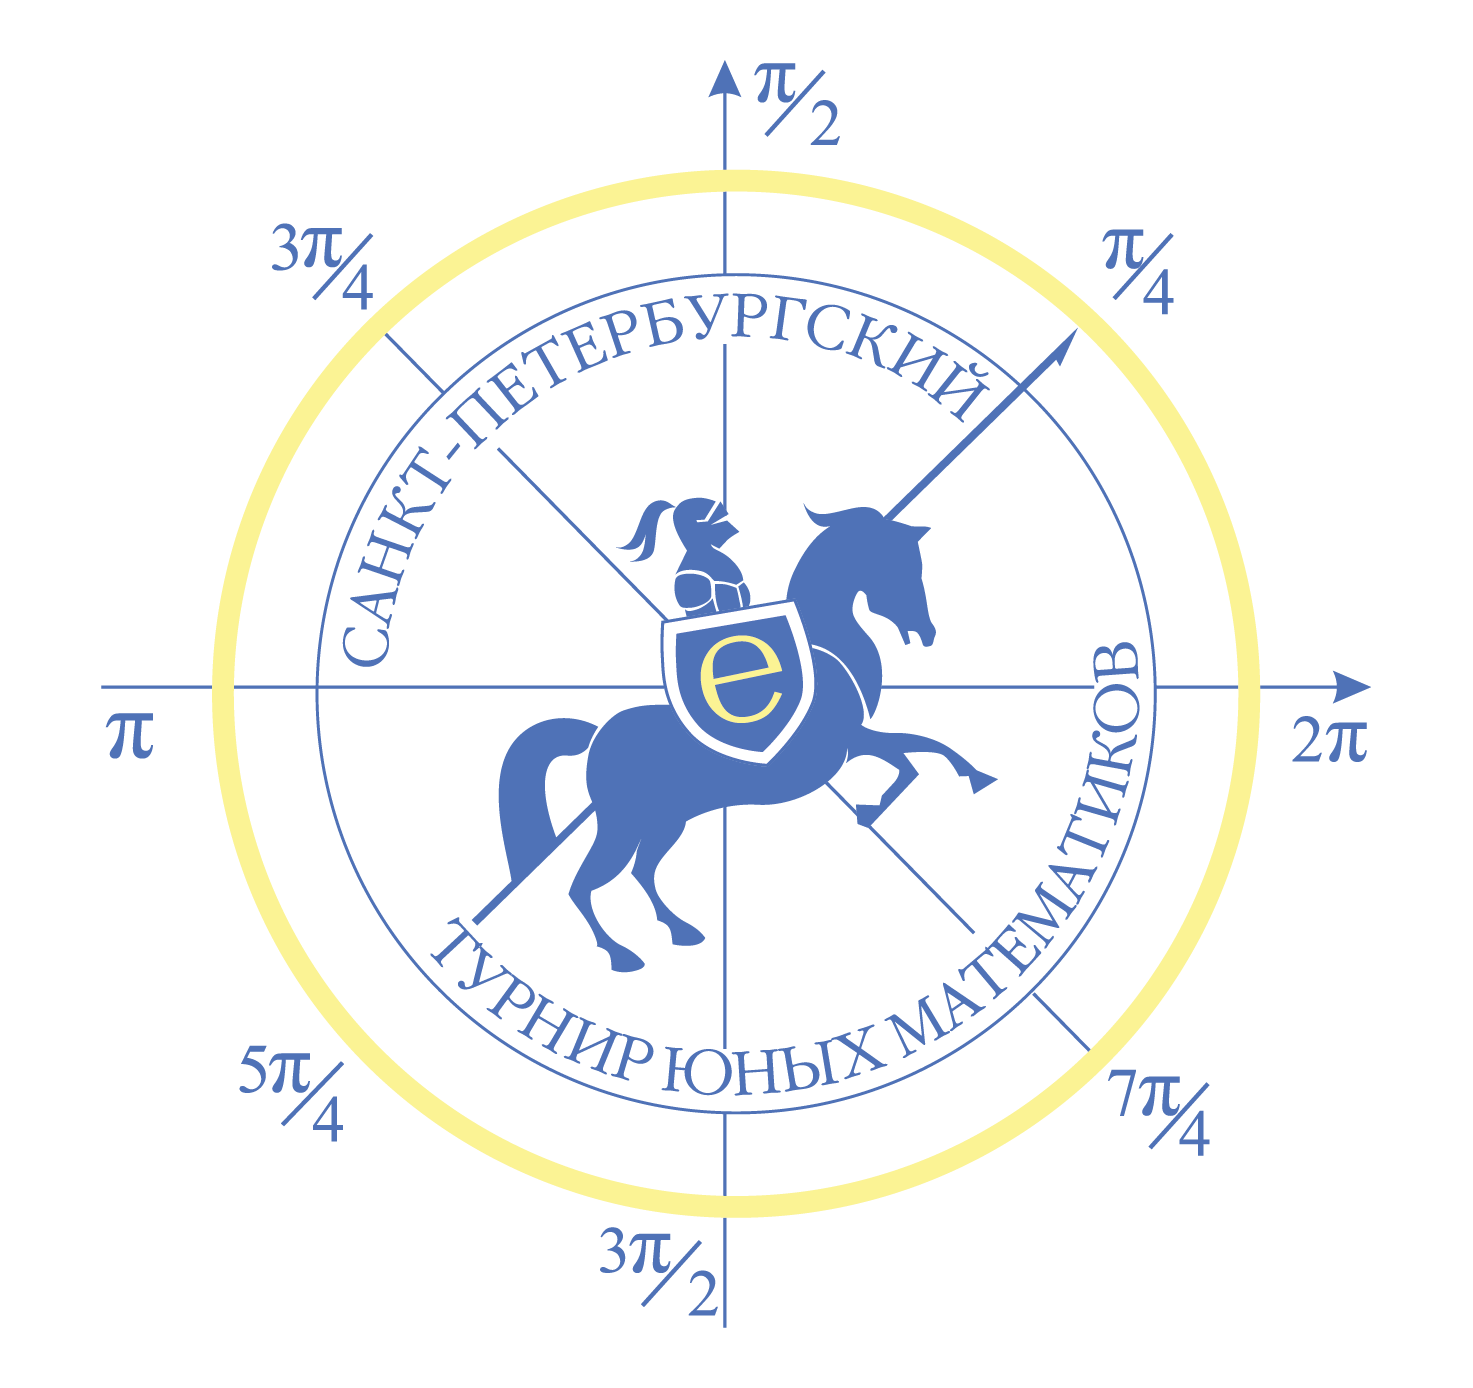
\includegraphics[width=0.3\textwidth]{TYM_logo.png}} &
\makecell[c]{
\includegraphics[width=0.3\textwidth]{fond_logo_hor}}
\end{tabular} \vspace{0.3cm}

    \large{Спасибо за внимание!} \vspace{0.5cm}
    
    Сайт Турнира: \myref{https://spbtym.ru/}{spbtym.ru} \vspace{1cm}
    
    Задать вопрос автору: \myref{mailto:todzhe@mail.ru}{todzhe@mail.ru}
\end{center}
}
\end{document}